\section{解的检验}
\label{sec:dsel-checks}

前三节都先用乘子或驻点“猜”出解的形式，再用一个恒等式验证它。实际计算中，候选分布还可能来自截断的级数、数值迭代或随机估计，它未必满足原问题的全部要求。拿到一个候选$\widehat{Q}$后，应当回到原问题依次回答三个问题：它是不是合法的候选，最小值存不存在，它是否达到了最小值或离最小值还有多远。图~\ref{fig:dsel-check-flow}把这些检查排成一条链。

\begin{BookInlineFigure}
 \centering
 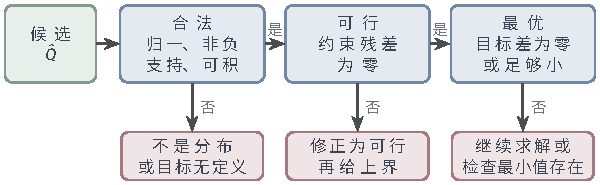
\includegraphics[width=102mm]{figures/07-probability/07-distribution-optimization/tikz/dsel-check-flow/figure.pdf}
 \caption{候选分布的检查顺序。绿框是待检的候选，蓝框是依次要通过的检查，红框是未通过时的处理：不合法的候选不能参加比较；不满足约束的候选先修正为可行分布，再用于给出最优值的上界；目标差不够小时继续求解，或回头检查最小值是否存在。}
 \label{fig:dsel-check-flow}
\end{BookInlineFigure}

\paragraph{候选是否合法}
第一步核对第~\ref{sec:dsel-problems}节列出的各项。归一化与非负性：指数形式的公式保证非负，但若配分函数是截断级数或数值积分得到的，归一化可能只是近似成立。支持：所有候选都要满足$\widehat{Q}\ll P$；倾斜公式自动满足，边界解则需要明确哪些状态的概率为零。可积性：目标与约束中的期望都要有限，下面会看到一个写得出公式、却因可积性失败而不合法的例子。

约束问题还要检查约束残差$\bm{r}=\mathbb{E}_{\widehat{Q}}[\bm{T}]-\bm{m}$。以第~\ref{sec:dsel-moment-matching}节Newton法的第一步为例，$\theta^{(1)}=9/14$给出
\[
 \widehat{Q}=Q_{\theta^{(1)}}\approx(0.1534,\ 0.2917,\ 0.5549),\qquad r\approx1.40147-1.42857=-0.0271 .
\]
它不满足约束，不属于可行集合。这时它的KL值$D_{\mathrm{KL}}(\widehat{Q}\Vert P)\approx0.1248$比真正的最优值$0.1429$还小，若把它当作“最小KL”报告就错了：违反约束的候选可以比最优解更好。

\paragraph{目标差}
不可行的倾斜分布并非没有用处。式~\eqref{eq:dsel-weak-duality}说明，任何$\bm{\theta}$都给出最优值的下界$\ell(\bm{\theta})$；再把$\widehat{Q}$修正成一个可行分布$\widetilde{Q}$，就得到上界$D_{\mathrm{KL}}(\widetilde{Q}\Vert P)$。两者之差
\begin{equation}
 D_{\mathrm{KL}}(\widetilde{Q}\Vert P)-\ell(\bm{\theta})\geq D_{\mathrm{KL}}(\widetilde{Q}\Vert P)-D^{*}\geq0
 \label{eq:dsel-certificate}
\end{equation}
控制了$\widetilde{Q}$离最优还差多少，这就是\term{最优性证书}（optimality certificate）：不必知道$D^{*}$，就能保证误差不超过一个算得出的数。

在例子中，$\widehat{Q}$的均值偏小，把它与均值最大的点质量$\delta_2$混合：
\[
 \widetilde{Q}=(1-\alpha)\widehat{Q}+\alpha\delta_2 ,
\]
均值为$(1-\alpha)\cdot1.40147+2\alpha$。令它等于$10/7$，解得
\[
 \alpha=\frac{10/7-1.40147}{2-1.40147}\approx0.04528 .
\]
修正后的$\widetilde{Q}\approx(0.1464,0.2785,0.5750)$可行，上界与下界分别为
\[
 D_{\mathrm{KL}}(\widetilde{Q}\Vert P)\approx0.143059,\qquad\ell(\theta^{(1)})=\frac{10}{7}\cdot\frac{9}{14}-A\Bigl(\frac9{14}\Bigr)\approx0.142234 .
\]
两者相差约$8.3\times10^{-4}$，所以$\widetilde{Q}$的KL离最优值不超过$8.3\times10^{-4}$，而最优值被夹在$[0.142234,\ 0.143059]$中。

对后续的Newton迭代点做同样的事，得到表~\ref{tab:dsel-certificate}与图~\ref{fig:dsel-certificate}。第二步之后证书已小于$2\times10^{-7}$，第三步约为$10^{-14}$，与数值舍入相当。

\begin{BookInlineTable}
 \centering
 \caption{Newton迭代点的最优性证书，$P$均匀，$T(x)=x$，$m=10/7$，精确最优值$D^{*}\approx0.1429124$。$\alpha$是为满足约束而混入$\delta_2$的比例。}
 \label{tab:dsel-certificate}
 \begin{tabular}{ccccc}
 \toprule
 $t$ & $\theta^{(t)}$ & 下界$\ell(\theta^{(t)})$ & 上界$D_{\mathrm{KL}}(\widetilde{Q}\Vert P)$ & 证书 \\
 \midrule
 $0$ & $0$ & $0$ & $0.170028$ & $1.7\times10^{-1}$ \\
 $1$ & $0.642857$ & $0.142234$ & $0.143059$ & $8.3\times10^{-4}$ \\
 $2$ & $0.692394$ & $0.1429122$ & $0.1429124$ & $1.8\times10^{-7}$ \\
 $3$ & $0.693147$ & $0.1429124$ & $0.1429124$ & $1.0\times10^{-14}$ \\
 \bottomrule
 \end{tabular}
\end{BookInlineTable}

\begin{BookInlineFigure}
 \centering
 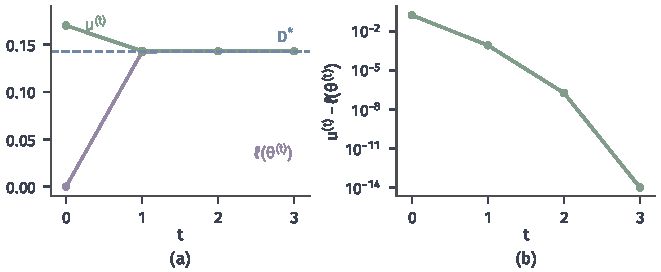
\includegraphics[width=112mm]{figures/07-probability/07-distribution-optimization/matplotlib/dsel-certificate/figure.pdf}
 \caption{最优性证书随Newton迭代的变化。(a)下界$\ell(\theta^{(t)})$（紫）与修正后可行分布的上界$u^{(t)}=D_{\mathrm{KL}}(\widetilde{Q}\Vert P)$（绿），蓝色虚线是$D^{*}$。(b)证书$u^{(t)}-\ell(\theta^{(t)})$，纵轴为对数刻度。}
 \label{fig:dsel-certificate}
\end{BookInlineFigure}

证书的两部分各有含义。在式~\eqref{eq:dsel-pythagoras-general}中分别取$Q=\widetilde{Q}$与$Q=Q^{*}$，得到
\[
 D_{\mathrm{KL}}(\widetilde{Q}\Vert P)-D^{*}=D_{\mathrm{KL}}(\widetilde{Q}\Vert Q^{*}),\qquad D^{*}-\ell(\bm{\theta})=D_{\mathrm{KL}}(Q^{*}\Vert Q_{\bm{\theta}}) .
\]
上界的误差是可行候选离最优分布的KL，下界的误差是最优分布离当前倾斜分布的KL。在第一步，两者约为$1.5\times10^{-4}$与$6.8\times10^{-4}$，和正是表中的$8.3\times10^{-4}$。

KL正则化的成本问题更直接。若$Z$能算出，最优值就是$-\tau\ln Z$，由式~\eqref{eq:dsel-gibbs-identity}，任何候选的目标差恰为$\tau D_{\mathrm{KL}}(\widehat{Q}\Vert Q^{*})$，不需要另找下界。

\paragraph{最小值是否存在}
有限状态上，可行集合非空时它是概率单纯形中的有界闭集，目标若在其上连续，最小值必然取到；第~\ref{sec:dsel-moment-matching}节的边界定理就是这样证明的。状态无穷时，这个论证会失效。

取$\mathcal{X}=\{1,2,\dots\}$，$P(k)=c/k^{3}$，$c=1/\sum_kk^{-3}\approx0.8319$。$P$的均值有限，
\[
 \mu=\mathbb{E}_{P}[X]=c\sum_{k\geq1}\frac1{k^{2}}=\frac{c\,\pi^{2}}{6}\approx1.3684 .
\]
要求$\mathbb{E}_{Q}[X]=2$，在可行分布中最小化$D_{\mathrm{KL}}(Q\Vert P)$。

先试倾斜。$q_\theta(k)\propto\mathrm{e}^{\theta k}/k^{3}$，当$\theta>0$时级数发散，倾斜分布不存在；当$\theta\leq0$时倾斜分布存在，但均值关于$\theta$不减（导数是方差），所以均值不超过$\theta=0$时的$\mu<2$。没有任何倾斜分布满足约束。

再看最优值。令$Q_N=(1-\varepsilon)P+\varepsilon\delta_N$，其中$\varepsilon=(2-\mu)/(N-\mu)$，它的均值是$\mu+\varepsilon(N-\mu)=2$，可行。$Q_N$与$P$的密度比在$k\neq N$处是$1-\varepsilon$，在$k=N$处是$1-\varepsilon+\varepsilon/P(N)$，所以
\[
 D_{\mathrm{KL}}(Q_N\Vert P)=(1-\varepsilon)\bigl(1-P(N)\bigr)\ln(1-\varepsilon)+Q_N(N)\ln\Bigl(1-\varepsilon+\frac{\varepsilon N^{3}}{c}\Bigr).
\]
第一项趋于零。第二项中$Q_N(N)\leq P(N)+\varepsilon$约为$0.632/N$，对数约为$2\ln N$，乘积约为$1.26\ln N/N$，也趋于零。数值上，$N=10,100,1000,10^{4}$时KL分别约为$0.261$、$0.0509$、$0.00793$、$0.00108$。所以最优值是$0$。

但最优值$0$达不到：$D_{\mathrm{KL}}(Q\Vert P)=0$只对$Q=P$成立，而$P$的均值是$1.3684$，不是$2$。图~\ref{fig:dsel-heavy-tail}画出这个机制：把极小的质量放到很远的地方，均值就能提高很多，KL的代价却微不足道。$Q_N$与$P$的总变差是$\varepsilon(1-P(N))\to0$，可是均值始终是$2$；函数$x$无界，均值不随分布的这种接近而连续变化，可行集合在这种收敛下不是闭的。

\begin{BookInlineFigure}
 \centering
 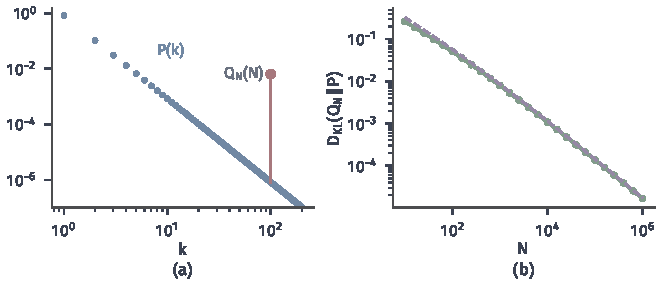
\includegraphics[width=112mm]{figures/07-probability/07-distribution-optimization/matplotlib/dsel-heavy-tail/figure.pdf}
 \caption{最小KL达不到的例子。$P(k)=c/k^{3}$，约束$\mathbb{E}_{Q}[X]=2$。(a)$P$的质量（蓝点），双对数坐标；$Q_{100}$把每项乘以$1-\varepsilon$，并在$k=100$处加上质量$\varepsilon\approx0.0064$（红）。(b)$D_{\mathrm{KL}}(Q_N\Vert P)$（绿）随$N$趋于零，紫色虚线是近似$\varepsilon\ln(\varepsilon N^{3}/c)$。}
 \label{fig:dsel-heavy-tail}
\end{BookInlineFigure}

一般空间中的存在性需要两方面的条件。一方面，KL的下水平集$\{Q:D_{\mathrm{KL}}(Q\Vert P)\leq a\}$在分布的弱收敛下是紧的，并且$D_{\mathrm{KL}}(\cdot\Vert P)$下半连续；证明需要用到下半连续函数的变分表示和第~\ref{chap:weak-convergence-of-distributions}章的胎紧性，可查阅~\scite{math-kallenberg2021probability}。另一方面，约束集合要在弱收敛下闭，例如$\bm{T}$有界连续时就是如此。两者都成立、且可行集合中有KL有限的分布时，最小值能取到。上面的例子缺的是第二条。

\paragraph{给出的分布是否达到最小值}
即使最优值有限、公式也写得出来，写出的分布仍可能不是候选。回到KL正则化的成本问题，取$\mathcal{X}=\{1,2,\dots\}$，$\tau=1$，
\[
 P(k)=c'\,\frac{\mathrm{e}^{-k}}{k^{2}},\qquad V(k)=-k ,
\]
其中$c'=1/\sum_k\mathrm{e}^{-k}k^{-2}\approx2.4465$。配分函数是
\[
 Z=\sum_{k\geq1}c'\frac{\mathrm{e}^{-k}}{k^{2}}\mathrm{e}^{k}=c'\frac{\pi^{2}}{6}\approx4.024 ,
\]
有限，Gibbs分布$Q^{*}(k)=\frac{6}{\pi^{2}k^{2}}$存在。可是
\[
 \mathbb{E}_{Q^{*}}\lvert V\rvert=\frac{6}{\pi^{2}}\sum_{k\geq1}\frac1k=\infty ,
\]
$Q^{*}$不在候选集合$\mathcal{Q}_V$中，定理~\ref{thm:dsel-gibbs-variational}的第二部分不适用。

第一部分仍然成立：对每个$Q\in\mathcal{Q}_V$，
\[
 J_1(Q)=-\ln Z+D_{\mathrm{KL}}(Q\Vert Q^{*})>-\ln Z ,
\]
严格不等号是因为$Q\neq Q^{*}$。另一方面，截断$Q_N=Q^{*}(\cdot\mid k\leq N)$只有有限个状态，属于$\mathcal{Q}_V$，并且
\[
 D_{\mathrm{KL}}(Q_N\Vert Q^{*})=-\ln Q^{*}(\{k\leq N\})\to0 .
\]
$N=10,100,1000$时它约为$0.060$、$0.0061$、$0.00061$。所以最优值是$-\ln Z\approx-1.392$，但没有候选达到它。只检查“公式里的$Z$有限”是不够的，还要检查公式给出的分布本身满足候选集合的可积性要求。

\paragraph{期望无法直接计算时}
上面的检查都需要计算期望：配分函数、矩、协方差、KL。状态数很大或空间连续时，这些量本身是难算的积分，常用随机抽样的平均来估计，估计值带有随机误差。这时约束残差与证书也只是估计：一个看起来很小的证书，可能只是估计误差掩盖了真实的差距。用抽样估计这些期望时，应当按第~\ref{chap:monte-carlo-integration-error}章的方法给出误差范围，并把它计入残差与证书，而不是只报告点估计。
